% Figure 3.1 (Session 3): the local Hilbert spaces and the Fock basis of three spinless orbitals.
% The image is rendered by figures/blender/s3_1_fock_basis.py; the coordinates of the labels
% come from figures/blender/out/fock_basis_anchors.tex. Compile with:
%   pdflatex fock_basis.tex ; result moves to ../many_body_fermions/fock_basis.pdf
\documentclass[11pt,tikz,border=0pt]{standalone}
\usepackage{amsmath,amssymb,graphicx}
\usepackage{xcolor}
\definecolor{coursedark}{HTML}{1B2A4A}
\definecolor{costamber}{HTML}{B8620A}
\newlength{\figw}\setlength{\figw}{16.19cm}   % the text width of the notes (letter, 2.7 cm margins), so labels print at size

\begin{document}
\begin{tikzpicture}[lbl/.style={font=\small, text=coursedark}]
  \node[anchor=south west, inner sep=0pt] at (0,0)
    {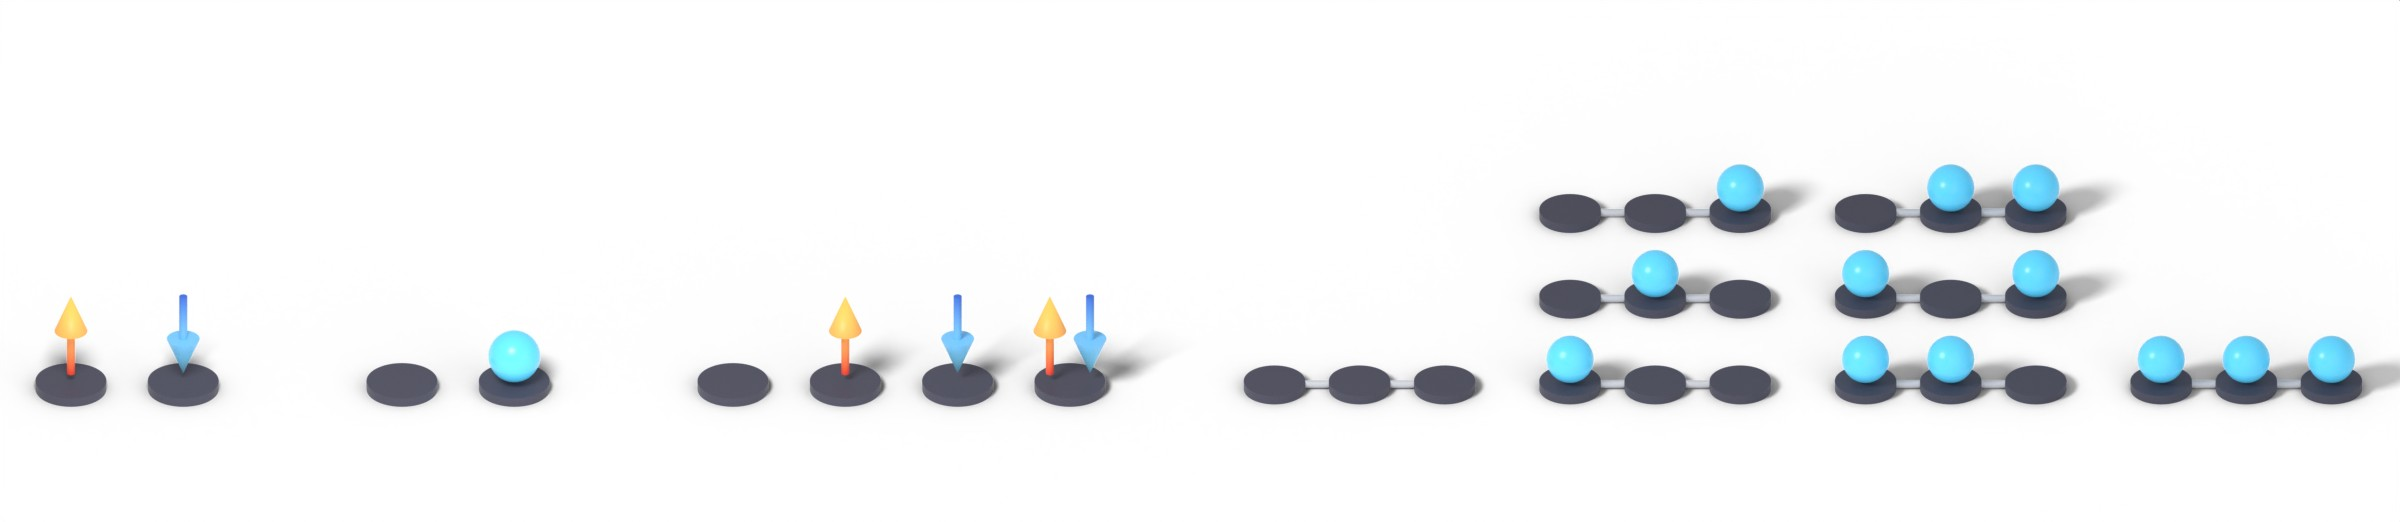
\includegraphics[width=\figw]{../blender/out/fock_basis.jpg}};
  %% written by figlib.py; x and y in units of the image width
\coordinate (spin) at (0.0530\figw,0.1493\figw);
\coordinate (spinN) at (0.0530\figw,0.0406\figw);
\coordinate (spinless) at (0.1909\figw,0.1493\figw);
\coordinate (spinlessN) at (0.1909\figw,0.0406\figw);
\coordinate (spinful) at (0.3756\figw,0.1493\figw);
\coordinate (spinfulN) at (0.3756\figw,0.0406\figw);
\coordinate (a) at (0.0049\figw,0.1695\figw);
\coordinate (N0) at (0.5665\figw,0.0419\figw);
\coordinate (N1) at (0.6897\figw,0.0419\figw);
\coordinate (N2) at (0.8128\figw,0.0419\figw);
\coordinate (N3) at (0.9360\figw,0.0419\figw);
\coordinate (b) at (0.5025\figw,0.1695\figw);
\coordinate (count) at (0.9828\figw,0.2261\figw);

  \node[lbl, font=\normalsize, anchor=west] at (a) {(a)};
  \node[lbl, font=\normalsize, anchor=west] at (b) {(b)};
  \node[lbl, anchor=north, align=center] at (spin) {spin-$\tfrac12$};
  \node[lbl, anchor=north, align=center] at (spinless) {spinless\\fermion};
  \node[lbl, anchor=north, align=center] at (spinful) {spinful\\fermion};
  \node[lbl, anchor=north] at (spinN) {$2^L$};
  \node[lbl, anchor=north] at (spinlessN) {$2^L$};
  \node[lbl, anchor=north] at (spinfulN) {$4^L$};
  \node[lbl, anchor=north] at (N0) {$N=0$};
  \node[lbl, anchor=north] at (N1) {$N=1$};
  \node[lbl, anchor=north] at (N2) {$N=2$};
  \node[lbl, anchor=north] at (N3) {$N=3$};
  \node[lbl, anchor=north east] at (count) {$1+3+3+1 = 2^3$};
\end{tikzpicture}
\end{document}
